\documentclass[10pt]{scrartcl}
\usepackage[latin1]{inputenc}
\usepackage[english, ngerman]{babel}
\usepackage[babel]{csquotes}
\usepackage{amsmath} % for eqref
\usepackage{tabularx}
\usepackage{pst-circ, pstricks-add}
\usepackage{graphicx}
\author{Denis Dietze \and Wolfgang Keller \and Nico Linke \and Thomas Schulte}

\title{Protokoll Einf?hrungsversuch E1}
\subtitle{Einsatz und Aufbau von Mess-- und Versorgungsger?ten}
\begin{document}
\maketitle

\section{Studienkontrollfragen}

\subsection{Aufbau und Funktion von Drehspul-- und Dreheisenmesswerken}

\subsubsection{Drehspulmesswerke}

In einem Drehspulmesswerk befindet ich im magnetischen Feld eines Dauermagneten\footnote{in modernen Ausf?hrungen befindet sich der Dauermagnet h?ufig \emph{innerhalb} der Spule und nicht au?erhalb; unter anderem weil hierdurch St?rfelder abgeschirmt werden} eine drehbare Spule. Spiralfedern sind leitend mit der Spule verbunden und dienen sowohl der Stromversorgung als auch der R?cksetzung in die Ruhelage.

Wird durch diese Spule Strom geleitet, so kommt es zur Wirkung der Lorentzkraft auf die Leiter der Spule. Diese dreht sich somit so weit, bis die Lorentzkraft gleich der winkelabh?ngigen R?ckstellkraft der Feder ist (was einen Ausschlag des Zeigers, der mit der Spule verbunden ist, bewirkt). Da die Federkraft nach dem Hooke'schen Gesetz proportional zur Auslenkung ist, folgt eine lineare Einteilung der Skala.

\subsubsection{Dreheisenmesswerke}

In einem \emph{Dreheisenmesswerk} befindet sich innerhalb einer Spule mit feststehendem Weicheisenkern ein an Federn befestigter drehbarer Kern (ein so genanntes "`Dreheisen"'), welcher ebenfalls aus Weicheisen besteht. An diesem inneren Kern ist ein Zeiger befestigt.

Wenn Strom durch die Spule geleitet wird, so kommt es zur Magnetisierung beider Eisenkerne und der drehbare innere Kern dreht sich so weit, bis die Federkraft gleich der magnetischen Absto?ungskraft ist. Da diese Auslenkung nicht proportional zur Stromst?rke ist, ist die Skala im Allgemeinen nichtlinear.

\subsection{Messbereichserweiterung an Strom-- und Spannungsmessern}

\subsubsection{Messbereichserweiterung an Strommessern}

Um den Messbereich von Strommessern zu erweitern, schaltet man einen Widerstand\emph{parallel} zum Messwerk. Seien $R_M$ bzw. $R_P$ die Widerst?nde von Messger?t bzw. Shunt und $I_M$ bzw. $I_P$ die durch Messger?t bzw. Parallelwiderstand flie?enden Str?me, sowie $I_{ges}=I_M+I_P$ der zu messende Strom.

Um den Messbereich n-fach zu erweitern, muss 
\begin{equation}
R_P=\frac{R_M}{n-1}
\label{eq:1}
\end{equation}
gew?hlt werden, da gilt:

\begin{displaymath}
\frac{I_P}{I_M}=\frac{R_M}{R_P}.
\end{displaymath}

Wenn man hier Gleichung \eqref{eq:1} einsetzt, folgt:
\begin{equation}
\frac{I_P}{I_M}=n-1.
\label{eq:2}
\end{equation}

Unter Beachtung von
\begin{displaymath}
I_{ges}=I_M+I_P
\end{displaymath}
folgt somit aus Gleichung \eqref{eq:2}:
\begin{displaymath}
I_{ges}=n I_M,
\end{displaymath}
was einer n-fachen Messbereichserweiterung entspricht.

\subsubsection{Messbereichserweiterung an Spannungsmessern}

Um den Messbereich von Spannungsmessern auf das n-fache zu erweitern, schaltet man einen Widerstand von $R_R=(n-1) R_M$ \emph{in Reihe} mit dem Spannungsmessger?t, wobei $R_M$ bzw. $R_R$ den Widerstand des Spannungsmessger?ts  bzw. in Reihe geschalteten Widerstands bezeichne. Stehe $U_M$ f?r die am Spannungsmesser anliegende Spannung und $U_M$ f?r die Summe der an Widerstand und Messger?t anliegenden Spannungen.

Mittels einer analogen Herleitung wie f?r die Messbereichserweiterung f?r Strommessger?te kann man zeigen, dass dann gilt:

\begin{displaymath}
U_{ges}=n U_M.
\end{displaymath}

\subsection{Stromrichtige vs. spannungsrichtige Messschaltung}

\subsubsection{Stromrichtige Messschaltung}

\begin{pspicture}%[showgrid=true]
(0, 0)(10,6)
    \pnode(1, 1){A}
    \pnode(1, 4){B}
    \pnode(3, 4){C}
    \pnode(7.5, 4){D}
    \pnode(7.5, 1){E}
    \pnode(3, 1){F}
    \battery(A)(B){$E$}
    \circledipole[labeloffset=0, tensionlabel=$U_A$](C)(D){A}
    \circledipole[labeloffset=0, tensionlabel=$E{=}U_A+U_{R_L}$, tensionlabeloffset=2.2](C)(F){V}
    \wire(B)(C)
    \resistor[tensionlabel=$U_{R_L}$, tensionlabeloffset=1.4](D)(E){$R_L$}
    \wire(E)(F)
    \wire(F)(A)
\end{pspicture}

\subsubsection{Spannungsrichtige Messschaltung}

\begin{pspicture}%[showgrid=true]
(0, 0)(9,6)
    \pnode(1, 1){A}
    \pnode(1, 4){B}
    \pnode(4, 4){C}
    \pnode(7.5, 4){D}
    \pnode(7.5, 1){E}
    \pnode(4, 1){F}
    \battery(A)(B){$E$}
    \circledipole[labeloffset=0, tensionlabel=$I_g{=}I_V+I_{R_L}$](B)(C){A}
    \circledipole[labeloffset=0, tensionlabel=$I_V$, tensionlabeloffset=1.4](C)(F){V}
    \wire(C)(D)
    \resistor[tensionlabel=$I_{R_L}$, tensionlabeloffset=1.4](D)(E){$R_L$}
    \wire(E)(F)
    \wire(F)(A)
\end{pspicture}

\subsubsection{Unterschiede zwischen stromrichtiger und spannungsrichtiger Messschaltung}

Bei der \emph{stromrichtigen Messschaltung} ist das Strommessger�t in Reihe mit dem Widerstand geschaltet, was zur Folge hat, dass der durch den Widerstand flie�ende Strom korrekt gemessen wird. Das Spannungsmessger�t befindet sich dagegen parallel zu einer Reihenschaltung aus Widerstand und Strommessger�t, mit der Folge dass als Spannung die Summe aus der am Strommessger�t anliegenden Spannung $U_A$ und der am Widerstand anliegenden Spannung $U_{R_L}$ gemessen wird, w�hrend wir "`eigentlich"' nur $U_{R_L}$ messen wollten. Es wird also bei dieser Messung eine h�here  Spannung gemessen, als am Widerstand anliegt.

Bei der \emph{spannungsrichtigen Messschaltung} dagegen ist das Spannungsmessger?t parallel zum Widerstand geschaltet. Die am Widerstand anliegende Spannung wird also korrekt gemessen. Das Strommessger?t befindet sich dagegen in Reihe mit einer Parallelschaltung aus dem Widerstand und dem Spannungsmessger?t. In der Folge wird die Summe der Str?me durch das Spannungsmessger?t $I_V$ und den Widerstand $I_{R_L}$ gemessen, w?hrend wir gerne den Strom durch den Widerstand messen w?rden - es wird also ein h?herer Strom gemessen als durch den Widerstand flie?t.

\subsection{Gesichtspunkte bei der Auswahl von Messger?ten}

\begin{itemize}
\item Gew?nschte Art der Messung (direkte Messung vs. indirekte (d. h. Messung anderer Gr??en, aus denen sich die gew?nschte Gr??e berechnet werden kann))
\item Messbereich
\item Empfindlichkeit des Messger�tes
\item Empfindlichkeit des Messger�ts in Bezug auf schnelle zeitliche �nderungen der Messgr��e
\end{itemize}

\subsection{Empfindlichkeit von Messger?ten}

Nach DIN 1319 versteht man unter der Empfindlichkeit eines Messger�ts die "`�nderung des Wertes der Ausgangsgr��e eines Messger�tes  bezogen auf die sie verursachende �nderung des Wertes der Eingangsgr��e"', also als Formel:
\begin{displaymath}
S = \frac{\Delta \alpha}{\Delta x},
\end{displaymath}
wobei $\alpha$ f�r den Wert der Ausgangsgr��e des Messger�ts (z. B. Zeigerausschlag) und x f�r den Wert der Eingangsgr��e steht.

\subsection{Fehlerarten bei Messungen}

Es gibt 2 Arten von Fehlern:
\begin{itemize}
\item Systemische Fehler
\item Zuf�llige Fehler
\end{itemize}

\emph{Systemische Fehler} sind Fehler, die (wenn sie identifiziert sind) nach Betrag und Vorzeichen quantifiziert werden k�nnen. Des weiteren sind sie reproduzierbar. Somit kann man, wenn sie erkannt und erfasst sind, die Messwerte um den entsprechenden Fehler korrigieren.

\emph{Zuf�llige Fehler} dagegen sind prinzipiell unvermeidbar. Sie k�nnen Betrag und Vorzeichen wechseln und sind nicht reproduzierbar. Sie behandelt man mit statistischen Methoden.

\subsection{Aufbau und Funktionsprinzip des Elektronenstrahloszilloskops}

\subsection{Frequenzmessung mittels Lissajousfiguren}

Die Entstehung der Figuren ist im Abschnitt \ref{abschnitt:liss} beschrieben. Um eine Frequenz mittels Lissajousfiguren zu messen, legt man an eine der beiden Achsen des Oszillographen die zu messenden Frequenz an und an die andere eine Referenzfrequenz.

Anschlie�end �ndert man die Referenzfrequenz so lange, bis auf dem Oszillographen eine Lissajous-Figur sichtbar wird, f�r die man das Frequenzverh�ltnis kennt.


\subsection{Das Prinzip der Whetstoneschen Messbr�cke}

\begin{pspicture}%[showgrid=true]
(1, 0)(9,7)
    \pnode(2, 1){A}
    \pnode(4, 1){B}
    \pnode(6, 1){C}
    \pnode(8, 1){D}
    \pnode(8, 3){E}
    \pnode(5, 3){F}
    \pnode(2, 3){G}
    \pnode(2, 6){H}
    \pnode(5, 6){I}
    \pnode(8, 6){J}
    \wire(A)(B)
    \battery(B)(C){$U=5~V$}
    \wire(C)(D)
    \wire(D)(E)
    \resistor(E)(F){$R_3$}
    \resistor(F)(G){$R_2$}
    \wire(G)(A)
    \circledipole[labeloffset=0, tensionlabel=$U_{Br}$, tensionlabeloffset=1.5](F)(I){V}
    \wire(D)(J)
    \wire(G)(H)
    \resistor(I)(J){$R_x$}
    \resistor[variable](H)(I){$R_1$}
\end{pspicture}

\section{Versuchsdurchf?hrung}

\subsection{Bestimmung der Widerstandswerte am Schiebewiderstand}

\subsubsection{Ergebnisse der Messung in stromrichtiger Messschaltung}

Die Ergebnisse der Messungen in stromrichtiger Messschaltung sind in Tabelle \ref{table:1} dargestellt.

\begin{table}
\begin{minipage}[t]{\textwidth}
\begin{center}
\begin{tabular}{|crrr|}
\hline
    Gew?hlte Klemmen & U \footnote{\label{fn:gemessen}gemessen} & I \footref{fn:gemessen} & R \footnote{aus gemessenem U und I berechnet; Genauigkeit zwei Dezimalstellen}\\
\hline
    1-2 & 5,1~V & 0,527~A & $9,68~\Omega$\\
    2-3 & 8,2~V & 0,508~A & $16,14~\Omega$\\
    1-3 & 8,2~V & 0,314~A & $26,11~\Omega$\\
\hline
\end{tabular}
\end{center}
\end{minipage}
\caption{Messergebnisse der Messung in spannungsrichtiger Messschaltung}
\label{table:1}
\end{table}

\subsubsection{Ergebnisse der Messung in spannungsrichtiger Messschaltung}

Die Ergebnisse der Messungen in stromrichtiger Messschaltung sind in Tabelle \ref{table:2} dargestellt.

\begin{table}
\begin{minipage}[t]{\textwidth} 
\begin{center} 
\begin{tabular}{|crrr|}
\hline
    Gew?hlte Klemmen & U \footnote{\label{fn:gemessen}gemessen} & I \footref{fn:gemessen} & R \footnote{aus gemessenem U und I berechnet; Genauigkeit zwei Dezimalstellen}\\
\hline
    1-2 & 5~V & 0,527~A & $9,49~\Omega$\\
    2-3 & 8,1~V & 0,508~A & $15,95~\Omega$\\
    1-3 & 8,1~V & 0,17~A & $47,65~\Omega$\\
\hline
\end{tabular}
\end{center}
\end{minipage}
\caption{Messergebnisse der Messung in stromrichtiger Messschaltung}
\label{table:2}
\end{table}

\subsubsection{Messung mittels Widerstandsmessger?ten}

Die Ergebnisse der Messungen sind in den Tabellen \ref{table:3} bis \ref{table:5} aufgelistet.

\begin{table}
\begin{minipage}[t]{\textwidth}
\begin{center}
\begin{tabular}{|cr|}
\hline
    Gew�hlte Klemmen & R %\footnote{\label{fn:gemessen}gemessen}
    \\
\hline
    1-2 & $10,8~\Omega$\\
    2-3 & $16,9~\Omega$\\
    1-3 & $27,5~\Omega$\\
\hline
\end{tabular}
\end{center}
\end{minipage}
\caption{Messergebnisse der direkten Widerstandsmessung mittels Digitalmultimeter VC 150}
\label{table:3}
\end{table}

\begin{table}
\begin{minipage}[t]{\textwidth}
\begin{center}
\begin{tabular}{|cr|}
\hline
    Gew�hlte Klemmen & R %\footnote{\label{fn:gemessen}gemessen}
    \\
\hline
    1-2 & $10,6~\Omega$\\
    2-3 & $17,0~\Omega$\\
    1-3 & $27,4~\Omega$\\
\hline
\end{tabular}
\end{center}
\end{minipage}
\caption{Messergebnisse der direkten Widerstandsmessung mittels Digitalvoltmeter G-1002.500}
\label{table:4}
\end{table}

\begin{table}
\begin{minipage}[t]{\textwidth}
\begin{center}
\begin{tabular}{|cr|}
\hline
    Gew�hlte Klemmen & R %\footnote{\label{fn:gemessen}gemessen}
    \\
\hline
    1-2 & $10.5~\Omega$\\
    2-3 & $17,2~\Omega$\\
    1-3 & $26,5~\Omega$\\
\hline
\end{tabular}
\end{center}
\end{minipage}
\caption{Messergebnisse der direkten Widerstandsmessung mittels Kleinme?br?cke nach Wheatstone bei einer Speisespannung von 5~V}
\label{table:5}
\end{table}

\subsection{Vergleich der Messergebnisse}

Die gemessenen bzw. aus den Messgr??en berechneten Widerst?nde sind in Tabelle \ref{table:6} abgetragen.

\begin{table}
\begin{minipage}[t]{\textwidth}
\begin{center}
\begin{tabularx}{\textwidth}{|Xrrrr|}
\hline
    Messger?t/--methode & $R_{1, 2}$  & $R_{2, 3}$ & $R_{1, 2}+R_{2, 3}$ & $R_{1, 3}$ \\
\hline
    Stromrichtige Messung & $9,68~\Omega$ & $16,14~\Omega$ &  $25,82~\Omega$ & $26,11~\Omega$ \\
    Spannungsrichtige Messung & $9,49~\Omega$ & $15,95~\Omega$ & $25,44~\Omega$ & $47,65~\Omega$ \\
    Direkte Widerstandmessung Digitalmultimeter VC 150 & $10,8~\Omega$ & $16,9~\Omega$ & $27,7~\Omega$ & $27,5~\Omega$ \\
    Direkte Widerstandsmessung Digitalvoltmeter G-1002.500 & $10,6~\Omega$ & $17,0~\Omega$ & $27,6~\Omega$ & $27,4~\Omega$ \\
    Direkte Widerstandsmessung Kleinme?br?cke nach Wheatstone & $10,5~\Omega$ & $17,2~\Omega$ & $27,7~\Omega$ & $26,5~\Omega$ \\
    Mittelwert aus allen Messungen\footnote{Messung von $R_{1,3}$ bei spannungsrichtiger Messung wurde aus der Mittelwertberechnung wegen offensichtlich fehlerhafter Messung herausgenommen} & $10,214~\Omega$ & $16,638~\Omega$ & $26,852~\Omega$ & $26.8775~\Omega$ \\
\hline
\end{tabularx}
\end{center}
\end{minipage}
\caption{Vergleich der Messergebnisse der angewendeten Messmethoden zur Widerstandsmessung}
\label{table:6}
\end{table}


Bei der au?erordentlich Abweichung f?r $R_{1, 2}+R_{2, 3}$ von $R_{1, 3}$ bei der spannungsrichtigen Messung gehen wir davon aus, dass ein Ablesefehler des Messger?tes vorlag. Speziell gehen wir f?r den Wert von 0,17~A (vgl. Tabelle \ref{table:1} bei der Messung des Stroms unter Verwendung der Messpunkte 1 und 3 davon aus, dass hier ein fehlerhafter Wert abgelesen oder aufgeschrieben wurde. Eine alternative Erkl?rung k?nnte ebenfalls sein, dass falsche Messpunkte verwendet wurden. Letztere Vermutung erh?lt dadurch eine gewisse Evidenz, als dass der ausgerechnete Wert f?r den Widerstand im Bereich des Doppelten des "`eigentlich"' zu messenden Wertes liegt. Bedingt durch den Aufbau des Widerstandes ist ein solcher Fehler durchaus m?glich. 

Abgesehen von diesem Messfehler l?sst sich der Unterschied zwischen strom- und spannungsrichtiger Messsung dadurch erkl?ren, als bei stromrichtiger Messung die Spannung leicht zu hoch gemessen wird (was gemessen wird ist $U_A+U_{R_L}$, was wir jedoch messen wollen ist $U_{R_L}$) und bei spannungsrichtiger Messung der Strom leicht zu hoch gemessen wird (gemessen wird $I_V+I_{R_L}$, was wir jedoch messen wollen ist $I_{R_L}$). Somit wird die aus $U_{R_L}$ und $I_{R_L}$ abgeleitete Gr??e $R_L$ bei stromrichtiger Messung untersch?tzt, denn es gilt:
\begin{displaymath}
R_L = \frac{U_{R_L}}{I_{R_L}} < \frac{U_{R_L}+U_A}{I_{R_L}}.
\end{displaymath}

Analog wird bei der spannungsrichtichtiger Messung die aus $U_{R_L}$ und $I_{R_L}$ abgeleitete Gr??e $R_L$ ?bersch?tzt, denn es gilt:
\begin{displaymath}
R_L = \frac{U_{R_L}}{I_{R_L}} > \frac{U_{R_L}}{I_{R_L}+I_V}.
\end{displaymath}

In der Tat zeigt der Vergleich der Messwerte von strom-- und spannungsrichtiger Messung (von dem "`groben Messfehler"' abgesehen), dass die aus den Messwerten berechneten Werte f?r den Widerstand in der Tat, wie aus der Theorie zu erwarten ist, bei der stromrichtigen Messung gr??er als bei der spannungsrichtigen Messung sind.

\subsection{Effektiv-- und Spitzenwermessung mittels verschiedener Messger?te}

Die gemessenen Spannung sind in Tabelle \ref{table:7} abgetragen.

\begin{table}
\begin{minipage}[t]{\textwidth}
\begin{center}
\begin{tabular}{|lr|}
\hline
    Messger?t & gemessene Spannung U \\
\hline
     Analogmultimeter 2010 & 1,8~V \\
     Digitalmultimeter VC 150 & 1,84~V \\
     Millivoltmeter MV 21 & 1,8~V \\
     Oszilloskop HM 203-7 & 5~V bzw. 2,5~V\footnote{ersterer Wert entspricht dem tats?chlich abgelesenen Wert f?r $\widehat{U}$ bzw. $U_{ss}$, letzterer entsteht durch Division des ersteren durch 2 und entspricht $U_s$}\\
\hline
\end{tabular}
\end{center}
\end{minipage}
\caption{Ermittelte Spannungswerte f?r verschiedene Messger?te bei $\widehat{U}=5~V$ und $f=1000~Hz$}
\label{table:7}
\end{table}

Das "`Analogmultimeter 2010"', das "`Digitalmultimeter VC 150"' und das "`Millivoltmeter MV 21"' stellen bei der Spannung den Effektivwert dar, w?hrend auf dem Oszilloskop (in diesem Fall vom Typ "`HM 203-7"') der Spitzenwert abgelesen werden kann.

Der Zusammenhang zwischen Effektivwert und Spitzenwert bei einer Sinusspannung ist
\begin{displaymath}
U_{eff} = \frac{1}{\sqrt{2}} U_s.
\end{displaymath}

\subsection{Oszillogramm einer Rechtecks-- und Sinusspannung}

\subsection{Frequenzmessung mit Hilfe von Lissajous-Figuren}

\label{abschnitt:liss}

Die Frequenzverh�ltnisse der Aufgabenstellung seien als $f_{y-Achse} : f_{x-Achse}$ zu betrachten. In den Abbildungen \ref{fig:0.5:1} bis \ref{fig:3:1} sind die in der Versuchsbeschreibung geforderten Skizzen der Lissajous-Figuren abgetragen.

Die Figuren entstehen folgenderma?en: an der x-- und y--Achse liegt je eine sinusf?rmige Spannung an:
\begin{eqnarray*}
u_x & = & U_s \sin (\frac{f_x}{2 \pi} t+\omega_x) \\
u_y & = & U_s \sin (\frac{f_y}{2 \pi} t+\omega_y),
\end{eqnarray*}
wobei $f_x, f_y$ f?r die entsprechenden Frequenzen und $\omega_x, \omega_y$ f?r die Phasenverschiebungen stehen. Da die Spitzenspannung an beiden Achsen im vorliegenden Experiment die selbe ist, wurde diese mit $U_s$ bezeichnet -- im Allgemeinen kann diese jedoch f?r x- und y-Achse unterschiedlich sein.

Da die Auslenkung des Oszillographen proportional zur Spannung ist, erh?lt man somit die Gleichung der Lissajous-Figuren

\begin{displaymath}
\left(
\begin{array}{c}
u_x \\ u_y
\end{array} \right) = U_s
\left(
\begin{array}{c}
\sin (\frac{f_x}{2 \pi} t+\omega_x) \\ \sin (\frac{f_y}{2 \pi} t+\omega_y)
\end{array}
\right)
\end{displaymath}

F?r $U_s=5~V$, Frequenzverh?ltnisse nach Aufgabenstellung und in den Diagrammen angegebenen Werten f?r $\omega_x$ und $\omega_y$ erh?lt die in den Abbildungen \ref{fig:0.5:1} bis \ref{fig:3:1} dargestellten Oszillogramme (bzw. mathematisch gesehen Trajektorien der angegebenen Kurvengleichung).

\begin{figure}
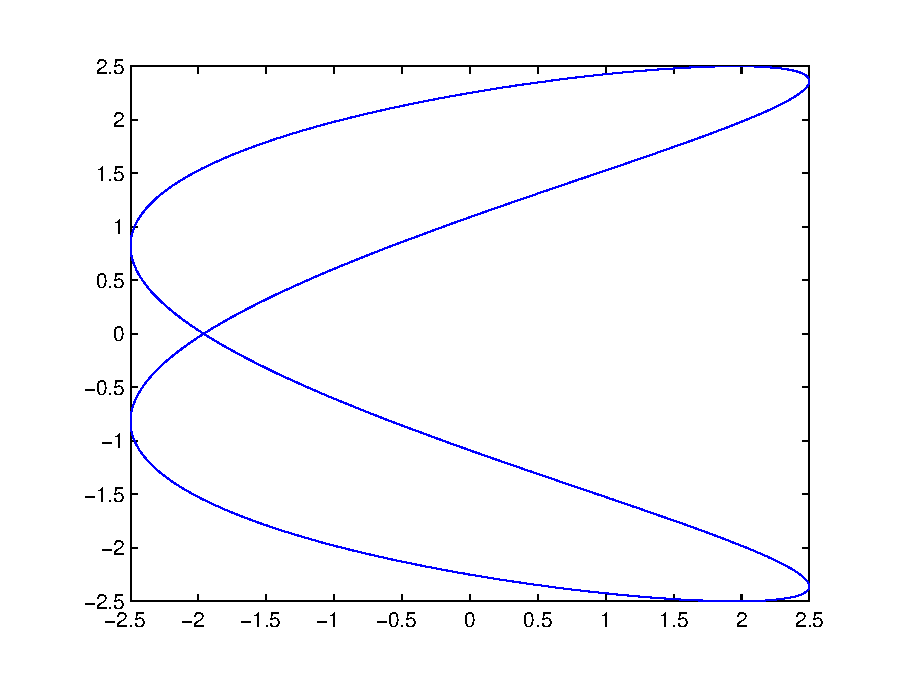
\includegraphics[width=0.5\textwidth]{05-1.eps}
\caption{Lissajous-Figur f?r Frequenzverh?ltnis 0.5:1, $\omega_x=0$ und $\omega_y=1.12$}
\label{fig:0.5:1}
\end{figure}

\begin{figure}
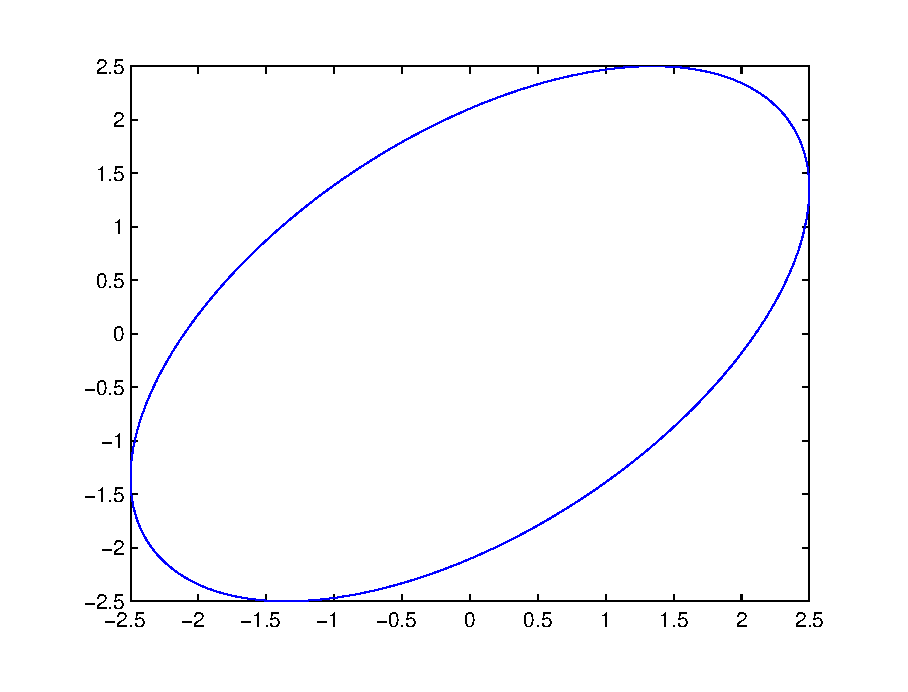
\includegraphics[width=0.5\textwidth]{1-1.eps}
\caption{Lissajous-Figur f?r Frequenzverh?ltnis 1:1, $\omega_x=0$ und $\omega_y=1$}
\label{fig:1:1}
\end{figure}

\begin{figure}
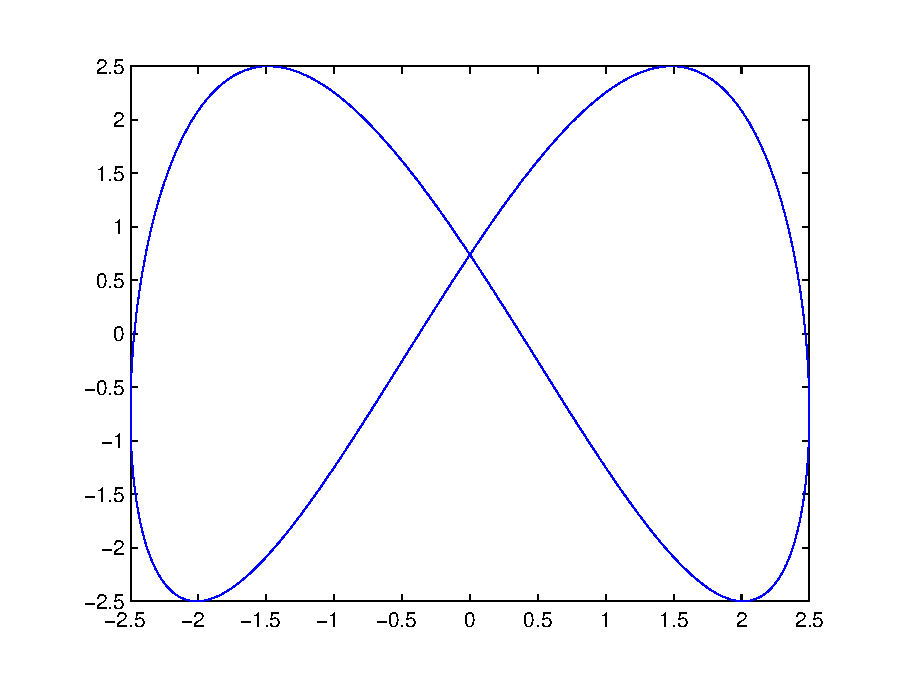
\includegraphics[width=0.5\textwidth]{2-1.eps}
\caption{Lissajous-Figur f?r Frequenzverh?ltnis 2:1, $\omega_x=0$ und $\omega_y=0.3$}
\label{fig:2:1}
\end{figure}

\begin{figure}
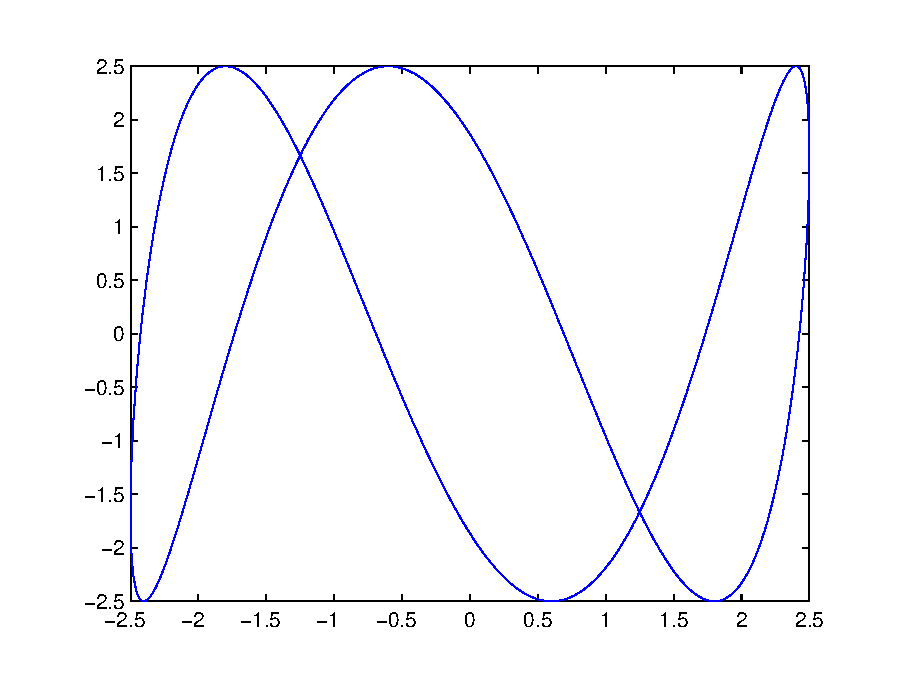
\includegraphics[width=0.5\textwidth]{3-1.eps}
\caption{Lissajous-Figur f?r Frequenzverh?ltnis 3:1, $\omega_x=0$ und $\omega_y=2.3$}
\label{fig:3:1}
\end{figure}

\end{document}